\documentclass{beamer}
\mode<presentation>
\usetheme{CambridgeUS}
\usepackage[russian]{babel}
\usepackage[utf8]{inputenc}
\usepackage[T2A]{fontenc}
%\usepackage{sansmathaccent}

\usepackage{verbatim}
\usepackage{alltt}

%\pdfmapfile{+sansmathaccent.map}
\title[СУБД]{Нормализация отношений}
\author{Наумов Д.А., доц. каф. КТ}
\date[14.03.2020] {Базы данных и базы знаний, 2020}

\begin{document}

%ТИТУЛЬНЫЙ СЛАЙД
\begin{frame}
  \titlepage
\end{frame}
  
%СОДЕРЖАНИЕ ЛЕКЦИИ
\begin{frame}
  \frametitle{Содержание лекции}
  \tableofcontents  
\end{frame}
  
%РАЗДЕЛ 1
\section{Типы приложений: транзакционная и аналитическая обработка}
\begin{frame}
OLTP (On-Line Transaction Processing) — интерактивная транзакционная обработка.
\begin{itemize}
\item запросы пользователей выполняются одновременно - 
обработка идёт в режиме реального или приближенного к реальному времени;
\item запросы представляют собой интенсивный поток коротких операций по вставке, изменению и удалению небольшого числа записей в БД;
\item большая часть запросов известна на этапе проектирования;
\item время выполнения сложных аналитических запросов не является критическим для системы;
\end{itemize}
Примеры OLTP-приложений:
\begin{itemize}
\item системы складского учета;
\item системы заказа билетов;
\item банковские системы;
\end{itemize}
Данные OLTP-приложений \textbf{сильно нормализованы}.
\end{frame}

\begin{frame}
OLAP (On-Line Analytical Processing) - интерактивная аналитическая обработка. 
\begin{itemize}
\item Данные находятся \textbf{в режиме чтения}, за исключением моментов их обновления.
\item Выборки представляют собой \textbf{одиночные тяжёлые запросы}: поиски и расчёты по множеству \textbf{произвольных} критериев.
\item \textbf{Время отклика системы не регламентировано}.
\item Размеры базы данных на порядок и больше транзакционных.
\end{itemize}
\begin{block}{Пример типовой архитектуры OLAP}
\begin{center}
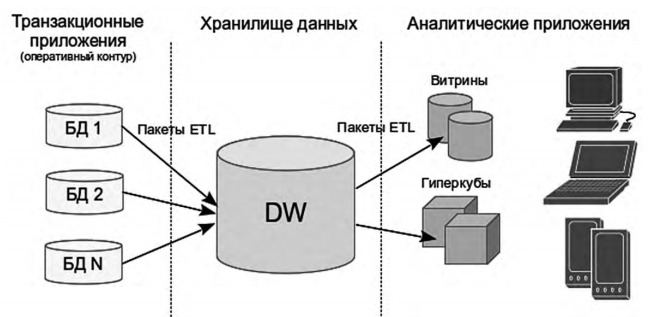
\includegraphics[scale=0.5]{images/olap.png}
\end{center}
\end{block}
\end{frame}

\section{Нормализация}
\begin{frame}
\begin{block}{Нормализация}
метод создания набора отношений с заданными свойствами на основе требований к данным, установленными в конкретной предметной области.
\end{block}
Цели нормализации:
\begin{itemize}
\item устранение избыточности при хранении данных, приводящей к увеличению размера БД.
\item исключение необходимости модификации данных в связных таблицах для минимизации времени и операций, проводящихся в одной транзакции.
\end{itemize}
Процесс нормализации:
\begin{enumerate}
\item исходная точка - представление предметной области в виде одного (или нескольких) отношений
\item на каждом шаге создается набор схем отношений, обладающих лучшими свойствами;
\item критерий <<лучше-хуже>> записит от целей проектирования.
\end{enumerate}
\end{frame}

\begin{frame}{Критерии оценки качества логичекой модели}
\begin{block}{Критерии оценки качества логичекой модели}
\begin{enumerate}
\item Адекватность базы данных предметной области.
\item Скорость выполнения операций обновления данных (вставка, обновление, удаление кортежей).
\item Скорость выполнения операций выборки данных.
\item Легкость разработки и сопровождения базы данных.
\item Отсутствие неоправданной избыточности данных.
\end{enumerate}
\end{block}
Критерии OLAP и OLTP:
\begin{itemize}
\item OLAP: на первый план выходит время отклика системы, данные могут быть избыточны.
\item OLTP: на первый план выходит обработка транзакций в режиме реального времени.
\end{itemize}
\end{frame}

\begin{frame}
\begin{block}{Избыточность данных}
одни и те же факты можно многократно получить из разных объектов базы данных
\end{block}
\begin{itemize}
\item польза: возможностm ускорения выполнения запросов;
\item избыточность должна быть контролируемой: необходима программная реализация проверок того, что избыточные и базовые данные адекватно согласованы между собой;
\end{itemize}
Расписание:
\begin{center}
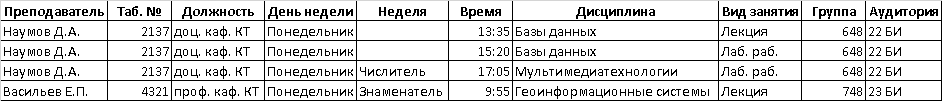
\includegraphics[scale=0.45]{images/ex-rasp-01.png}
\end{center}
Должности:
\begin{center}
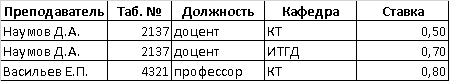
\includegraphics[scale=0.45]{images/ex-rasp-02.png}
\end{center}
\end{frame}

\begin{frame}
\begin{block}{Основные свойства нормальных форм}
\begin{itemize}
\item каждая следующая нормальная форма в некотором смысле улучшает свойства предыдущей;
\item при переходе к следующей нормальной форме свойства предыдущих нормальных форм сохраняются;
\end{itemize}
\end{block}
\begin{center}
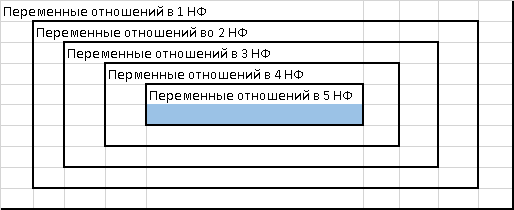
\includegraphics[scale=0.75]{images/forms.png}
\end{center}
\end{frame} 

\begin{frame}
\begin{block}{Схемы БД называются эквивалентными}
если содержание исходной БД может быть получено путем эквивалентного соединения отношений, входящих в результирующую схему, и при этом не появляется новых кортежей.
\end{block}
Исходная схема отношения:
\begin{center}
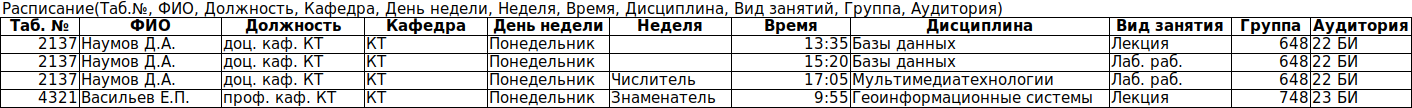
\includegraphics[scale=1.0]{images/ex-rasp-03.png}
\end{center}
Эквивалентная схема, полученная путем декомпозиции на два отношения:
\begin{center}
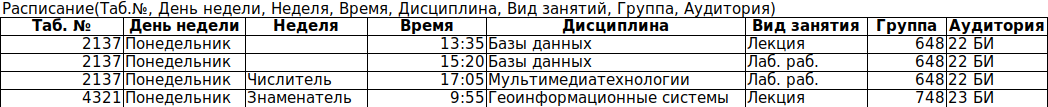
\includegraphics[scale=1.2]{images/ex-rasp-04.png}
\end{center}
\begin{center}
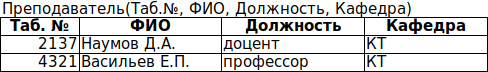
\includegraphics[scale=1.2]{images/ex-rasp-05.png}
\end{center}
\end{frame} 

\begin{frame}
\begin{block}{1НФ - первая нормальная форма}
выполняется, если все значения атрибутов (колонок таблицы) атомарны, то есть неделимы.
\end{block}
\begin{itemize}
\item cобственные типы данных СУБД считаются атомарными, исключение
могут составлять массивы, в том числе символьные (текстовые) и байтовые.
\item атомарность может быть относительна выбранного взгляда со стороны предметной области и контекста. 
\end{itemize}
Примеры:
\begin{itemize}
\item телефонный номер (в базе данных маркетинга, у телефонных операторов);
\item колонки для хранения комментариев;
\item целая и дробная части действительного числа, дата-время;
\item фамилия, имя, отчество в одной колонке.
\end{itemize}
\begin{center}
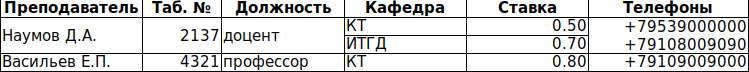
\includegraphics[scale=1.5]{images/ex-rasp-06.png}
\end{center}
\end{frame} 

\begin{frame}
\begin{block}{Переменная отношения находится в 2НФ}
тогда и только тогда, когда она находится в первой нормальной форме и каждый неключевой атрибут неприводимо зависит от (каждого) её потенциального ключа
\end{block}
\begin{itemize}
\item \textbf{Неприводимость}: в составе потенциального ключа отсутствует меньшее подмножество атрибутов, от которого можно также вывести данную функциональную зависимость.
\item Если потенциальный ключ является составным, то в отношении не должно быть неключевых атрибутов, зависящих от части составного потенциального ключа. 
\end{itemize}
\begin{center}
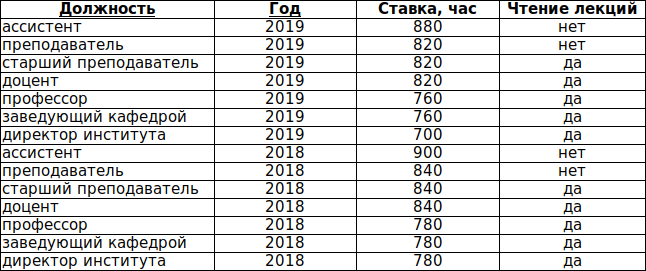
\includegraphics[scale=1.4]{images/ex-rasp-07.png}
\end{center}
\end{frame}

\begin{frame}
Отношение \textbf{Ставки}(\underline{Должность, Год}, Ставка, Чтение лекций)
\begin{center}
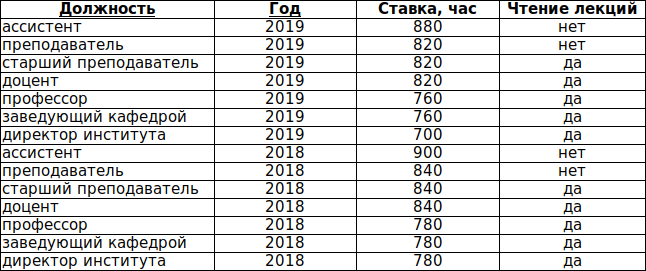
\includegraphics[scale=1]{images/ex-rasp-07.png}
\end{center}
Ключи и функциональные зависимости:
\begin{itemize}
\item ключ: \underline{Должность, Год}
\item функциональная зависимость: Должность, Год $\rightarrow$ Ставка
\item функциональная зависимость: Должность $\rightarrow$ Чтение лекций
\end{itemize}
Нарушение второй нормальной формы: атрибут функционально зависит от части первичного ключа.

Декомпозиция:
\begin{itemize}
\item отношение \textbf{Ставки}(\underline{Должность, Год}, Ставка)
\item отношение \textbf{Должности}(\underline{Должность}, Чтение лекций)
\end{itemize}
\end{frame}

\begin{frame}
\begin{block}{Переменная отношения находится в 3НФ}
тогда и только тогда, когда для каждой из её функциональных зависимостей X $\rightarrow$ A выполняется хотя бы одно из следующих условий: 
\begin{itemize}
\item Х содержит А (то есть X $\rightarrow$ A - тривиальная функциональная зависимость);
\item Х - суперключ;
\item А - ключевой атрибут (А входит в состав потенциального ключа).
\end{itemize}
\end{block}
Пример: продажа каждой товарной позиции имеет своим основанием документ (заказ, счёт и т.д.), а её стоимость характеризуется ценой, количеством и валютой.

Транзитивные зависимости:
\begin{itemize}
\item Идентификатор продажи $\rightarrow$ Номер документа
\item Идентификатор продажи $\rightarrow$ Код валюты
\item Номер документа $\rightarrow$ Код валюты
\end{itemize}
\end{frame}

\begin{frame}
Пример: \textbf{Студент}(\underline{№ зачетки}, ФИО, Группа, Факультет, Специальность, Выпускающая кафедра)
\begin{block}{Функциональные зависимости}
\begin{itemize}
\item № зачетки $\rightarrow$ ФИО, Группа, Факультет, Специальность, Выпускающая кафедра
\item Группа $\rightarrow$ Факультет, Специальность, Выпускающая кафедра
\item Выпускающая кафедра $\rightarrow$ Факультет
\end{itemize}
\end{block}
\begin{block}{Итоговые отношения}  
\begin{itemize}
\item \textbf{Студенты} (\underline{№ зачетки}, ФИО, Группа)
\item \textbf{Группы} (\underline{Группа}, Специальность, Выпускающая кафедра)
\item \textbf{Выпускающие кафедры} (\underline{Выпускающая кафедра}, Факультет)
\end{itemize}
\end{block}
\end{frame}

\begin{frame}
\begin{block}{Функциональная зависимость}
Пусть R является переменной отношения, а X и Y — произвольными подмножествами множества атрибутов переменной отношения R. Y функционально зависимо от X тогда и только тогда, когда для любого допустимого значения переменной отношения R, если два кортежа переменной отношения R совпадают по значению X, они также совпадают и по значению Y.
\end{block}
\begin{itemize}
\item Подмножество X - \textbf{детерминант}, а Y - \textbf{зависимая часть}.
\item Функциональная зависимость \textbf{тривиальна} тогда и только тогда, когда её правая (зависимая) часть является подмножеством её левой части (детерминанта).
\item Функциональная зависимость называется \textbf{неприводимой слева}, если ни один атрибут не может быть опущен из её детерминанта без нарушения зависимости (иными словами, детерминант неизбыточен). 
\end{itemize}
\end{frame}

\begin{frame}
\begin{block}{Переменная отношения находится в НФБК}
тогда и только тогда, когда каждая её нетривиальная и неприводимая слева функциональная зависимость имеет в качестве своего детерминанта некоторый потенциальный ключ
\begin{itemize}
\item НФБК - нормальная форма Бойса-Кодда;
\item менее строгое определение: детерминанты всех её функциональных зависимостей являются потенциальными ключами.
\end{itemize}
\end{block}
Ситуация, когда отношение будет находиться в 3НФ, но не в НФБК:
\begin{itemize}
\item отношение имеет два (или более) потенциальных ключа, которые являются составными
\item между отдельными атрибутами таких ключей существует функциональная зависимость
\end{itemize}
Поскольку описанная зависимость не является транзитивной, то такая ситуация под определение 3НФ не подпадает. 
\end{frame}

\begin{frame}
Отношение \textbf{Учебные пары}(Номер, Время начала, Время окончания, Смена)
\begin{center}
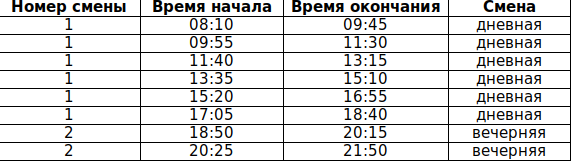
\includegraphics[scale=1]{images/ex-rasp-08.png}
\end{center}
Потенциальные ключи:
\begin{itemize}
\item Номер пары, Время начала
\item Номер пары, Время окончания
\item Смена, Время начала
\item Смена, Время окончания
\end{itemize}
Свойства отношения:
\begin{itemize}
\item Требования второй нормальной формы выполняются, так как все атрибуты входят в какой-то из потенциальных ключей, а неключевых атрибутов в отношении нет.
\item Также нет и транзитивных зависимостей, что соответствует требованиям третьей нормальной формы.
\item Cуществует функциональная зависимость Номер пары $\rightarrow$ Смена, в которой левая часть (детерминант) не является потенциальным ключом отношения, то есть отношение не находится в нормальной форме Бойса — Кодда.
\end{itemize}
\end{frame}

\begin{frame}
Отношение \textbf{Учебные пары}(Номер, Время начала, Время окончания, Смена)
\begin{center}
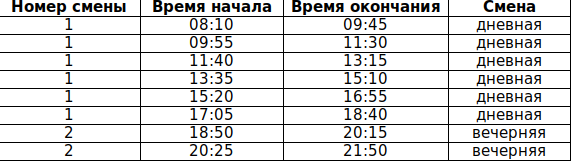
\includegraphics[scale=1]{images/ex-rasp-08.png}
\end{center}
Нормализованные отношения:
Отношение \textbf{Учебные пары}(Номер, Время начала, Время окончания)
\begin{center}
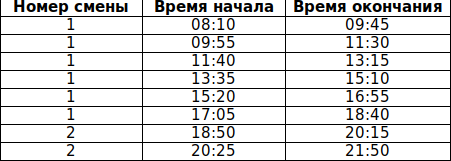
\includegraphics[scale=1]{images/ex-rasp-09.png}
\end{center}
Отношение \textbf{Смены}(Номер, Смена)
\begin{center}
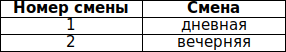
\includegraphics[scale=1]{images/ex-rasp-10.png}
\end{center}
\end{frame}

\begin{frame}
\begin{block}{Многозначная зависимость}
Пусть существует некоторое отношение $r$ со схемой $R$, а также два произвольных подмножества атрибутов $A,B\subseteq R$. Пусть $C \overset (A\cup B)$.
В этом случае $B$ многозначно зависит от $A$, тогда и только тогда, когда множество значений атрибута $B$, соответствующее заданной паре $[a:A;c:C]$ отношения $r$, зависит от $a$ и не зависит от $c$. 
\end{block}
\begin{block}{4НФ}
Переменная отношения R находится в четвёртой нормальной форме, если она находится в НФБК и все нетривиальные многозначные зависимости фактически являются функциональными зависимостями от её потенциальных ключей. 
\end{block}
\end{frame}

\begin{frame}
Отношение \textbf{Дисциплины студентов}(Студент, Группа, Дисциплина)
\begin{center}
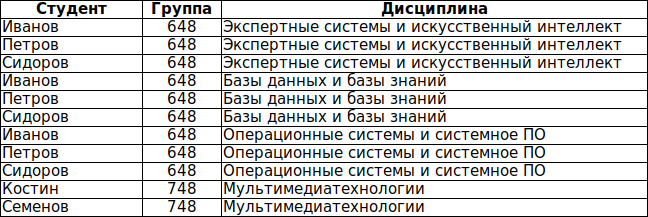
\includegraphics[scale=1]{images/ex-rasp-11.png}
\end{center}
\begin{itemize}
\item переменная отношения не соответствует 4НФ, так как существует следующая многозначная зависимость: Группа $\twoheadrightarrow$ Студент, Группа $\twoheadrightarrow$ Дисцилина
\item при добавлении нового студента в группу придется ему добавлять список изучаемых его группой дисциплин.
\end{itemize}
Нормализованные отношения:
Отношение \textbf{Группы}(Группа, Студент)
\begin{center}
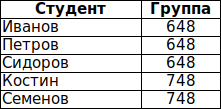
\includegraphics[scale=1]{images/ex-rasp-12.png}
\end{center}
Отношение \textbf{Дисциплины}(Группа, Дисциплина)
\begin{center}
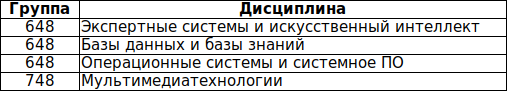
\includegraphics[scale=1]{images/ex-rasp-13.png}
\end{center}
Если к исходной переменной отношения добавить атрибут, функционально зависящий от потенциального ключа, например оценку по дисциплине  учётом стоимости доставки (Студент, Группа, Дисциплина - Оценка), то полученное отношение будет находиться в 4НФ и его уже нельзя подвергнуть декомпозиции без потерь.
\end{frame}

\begin{frame}
Допустимые схемы для OLAP: "снежинка", "звезда":
\begin{itemize}
\item центральным элементом являются таблицы фактов, содержащие события, транзакции, документы и др.
\item в таблице фактов одному документу (каждой его строке), соответствует одна запись.
\end{itemize}
\begin{block}{Денормализация документов в таблицу фактов}
\begin{center}
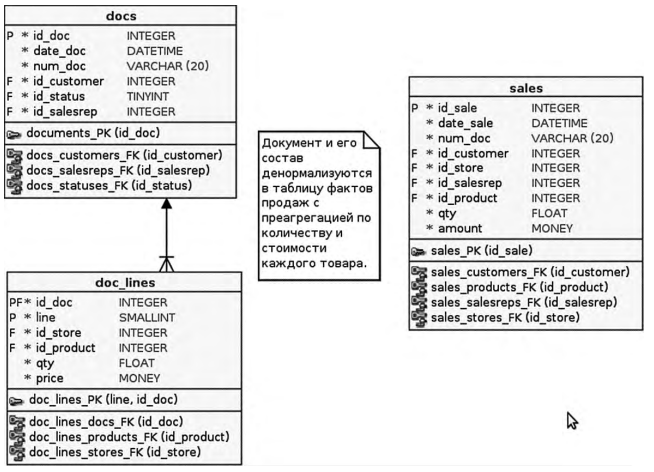
\includegraphics[scale=0.4]{images/denorm.png}
\end{center}
\end{block}
\end{frame}

\begin{frame}
\begin{block}{Пример SQL-запроса в транзакционной СУБД}
\begin{center}
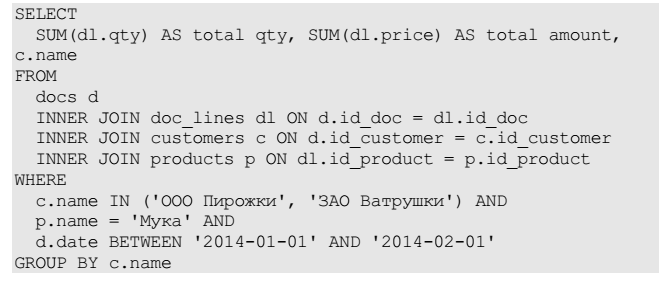
\includegraphics[scale=0.45]{images/sql-trans.png}
\end{center}
\end{block}
\begin{block}{Пример SQL-запроса в OLAP-СУБД}
\begin{center}
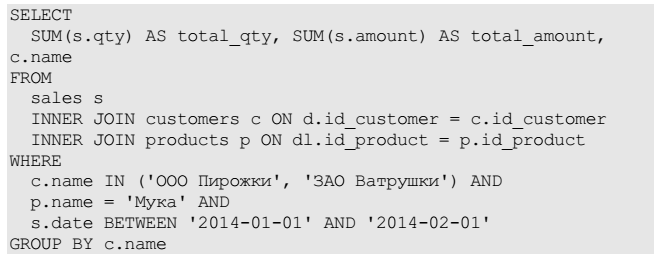
\includegraphics[scale=0.45]{images/sql-analitic.png}
\end{center}
\end{block}
\end{frame}

\begin{frame}
Если таблица фактов ссылается на таблицы-измерения, имеющие ссылки на другие измерения, то такая схема называется "снежинка".
\begin{block}{Таблица фактов в схеме "снежинка"}
\begin{center}
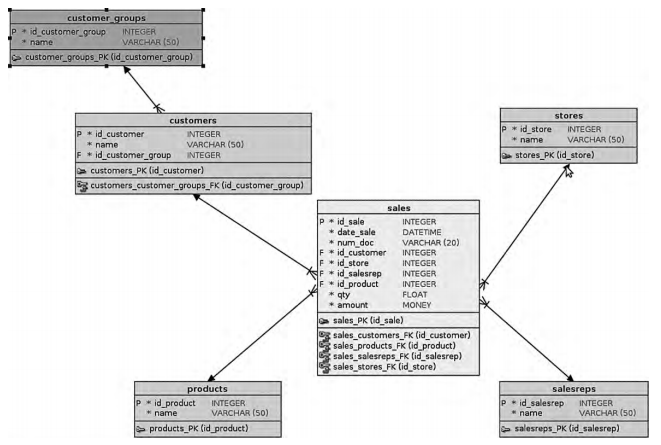
\includegraphics[scale=0.45]{images/snow.png}
\end{center}
\end{block}
Для запросов, включающих фильтрацию по группам клиентов, приходится делать дополнительное соединение.
\end{frame}

\begin{frame}
Схема "Звезда" полностью исключает иерархию измерений и необходимость соединения соответствующих таблиц в одном запросе.
\begin{block}{Таблица фактов в схеме "звезда"}
\begin{center}
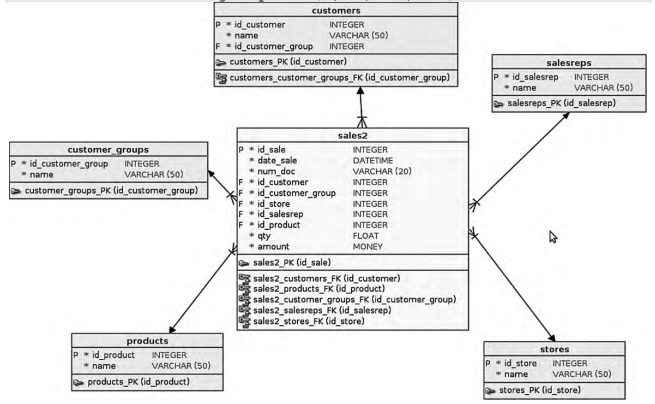
\includegraphics[scale=0.45]{images/star.png}
\end{center}
\end{block}
Обратной стороной денормализации всегда является избыточность, являющаяся причиной увеличения размера БД как в случае транзакционных, так и аналитических приложений.
\end{frame}


\begin{frame}
\begin{block}{Пример SQL-запроса в схеме "снежинка"}
\begin{center}
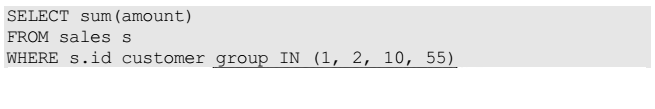
\includegraphics[scale=0.5]{images/star-sql.png}
\end{center}
\end{block}
\begin{block}{Пример SQL-запроса в схеме "звезда"}
\begin{center}
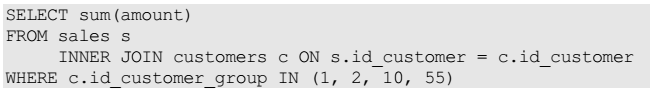
\includegraphics[scale=0.5]{images/snow-sql.png}
\end{center}
\end{block}
\begin{block}{Задача}
Посчитаем, примерную дельту на приведённом выше примере преобразования
"снежинки" в "звезду", если таблица продаж не использует компрессию данных и содержит
около 500 миллионов строк, а количество групп покупателей порядка 1000.
\end{block}
\end{frame}

\begin{frame}
\begin{itemize}
\item \textbf{теория нормализации является очень ценным достижением реляционной теории и практики}, поскольку она даёт научно строгие и обоснованные критерии качества проекта БД и формальные методы для усовершенствования этого качества;
\item идеи нормализации \textbf{полезны} для проектирования баз данных, они отнюдь н\textbf{е являются универсальным или исчерпывающим средством} повышения качества проекта БД - что существует слишком большое разнообразие возможных ошибок и недостатков в структуре БД, которые нормализацией не устраняются;
\item во всей сфере информационных технологий практически \textbf{отсутствуют методы оценки и улучшения проектных решений}, сопоставимые с \textbf{теорией нормализации реляционных баз данных} по уровню формальной строгости.
\end{itemize}
\end{frame} 

\end{document}